\documentclass[a4paper, 10pt, final, garamond]{book}
\usepackage{cours-preambule}
\graphicspath{{./figures/}}
\addto\captionsfrench{\renewcommand{\figurename}{Fig.}}

\makeatletter
\renewcommand{\@chapapp}{Contr\^ole de connaissances}
\makeatother

% \toggletrue{student}
% \toggletrue{corrige}
\renewcommand{\mycol}{black}
% \renewcommand{\mycol}{gray}

\hfuzz=5.003pt

\begin{document}
\setcounter{chapter}{5}

\settype{enon}
\settype{solu}

\chapter{Électrocinétique~: ressort amorti\ifstudent{~(15')}}

\vspace{-15pt}
\begin{enumerate}[label=\sqenumi, leftmargin=10pt]
	\item[n]{24}
	      \noindent
	      \begin{minipage}[t]{.65\linewidth}
		      On suppose le système mécanique suivant, constitué du point M de masse
		      $m$ accroché à un ressort idéal $(k,\ell_0)$ mais subissant des
		      frottements fluides. On travaille dans le référentiel $\Rc\ind{sol}$
		      supposé galiléen, avec le repère $(\Or, \ux, \uy)$. On suppose le
		      ressort initialement étiré tel que $\ell(0) = L_0 > \ell_0$, lâché
		      sans vitesse initiale.
	      \end{minipage}
	      \hfill
	      \begin{minipage}[t]{.32\linewidth}
		      ~
		      \vspace{-40pt}
		      \begin{center}
			      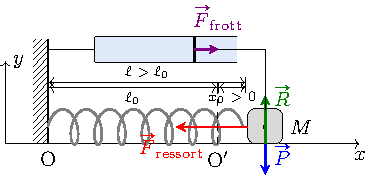
\includegraphics[width=\linewidth]{ressort_amorti}
			      % \vspace*{-10pt}
			      % \captionof{figure}{}
		      \end{center}
	      \end{minipage}
	      Effectuer un \textbf{bilan des forces} puis déterminer
	      l'\textbf{équation différentielle sous forme canonique} de
	      $\mathbf{\ell(t)}$ pour $t \geq 0$, et la réécrire en effectuant un
	      \textbf{changement de variable}. Déterminer les \textbf{expressions de}
	      $\mathbf{\w_0}$ et $\mathbf{Q}$, puis \textbf{résoudre} l'équation
	      différentielle sur le \textbf{changement de variable} pour un régime
	      \textbf{pseudo-périodique}. On appelle $x_0 = L_0 - \ell_0$.
	      % \smallbreak
	      Exprimer la \textbf{période $\mathbf{T}$ des oscillations amorties} en
	      fonction de $Q$ et de la \textbf{période} $\mathbf{T_0}$ des
	      oscillations harmoniques, donner \textit{sans démonstration}
	      l'\textbf{approximation de} $\mathbf{t_{95}}$ et \textbf{tracer la
		      solution}, avec $\mathbf{Q \approx 3}$.
	      \smallbreak
	      \vspace{-05pt}
	      \begin{isd}[sidebyside align=top]
		      \psw{%
			      \begin{itemize}
				      \item[b]{Bilan des forces~:} \hspace{12pt} \pt{1} + \pt{1}
				            \[
					            \begin{array}{ll}
						            \textbf{Poids}               & \Pf = m\gf = -mg \uy   \\
						            \textbf{Réaction normale}    & \Rf = R\uy             \\
						            \textbf{Force de rappel}     &
						            \Ff_r = -k (\ell(t) - \ell_0)\ux                      \\
						            \textbf{Force de frottement} & \Ff_{f} = -\alpha\vf =
						            -\alpha \dv{\ell}{t} \ux
					            \end{array}
				            \]
			      \end{itemize}
			      Avec le PFD~:
			      \begin{DispWithArrows*}[fleqn, mathindent=0pt, groups]
				      m\af &\stm{=} \Pf + \vv{R} + \Ff_{r} + \Ff_{f}
				      \Arrow{Dvlp$^{\xul{\rm t}}$}
				      \\
				      \Lra m\left(
				      \begin{array}{c}
						      \dv[2]{\ell}{t} \\
						      0
					      \end{array}
				      \right)
				      &=
				      \left(
				      \begin{array}{c}
						      -k (\ell(t) - \ell_0) -\alpha \dv{\ell}{t} \\
						      -mg + R
					      \end{array}
				      \right)
			      \end{DispWithArrows*}
			      Donc sur l'axe $\ux$
			      \begin{DispWithArrows*}[fleqn, mathindent=0pt, groups]
				      % \Arrow{$\cdot \ux$}
				      m \dv[2]{\ell}{t} + \alpha \dv{\ell}{t} + k\ell &\stm{=} k \ell_0
				      \CArrow{$\mdiv m$}
				      \\\Lra
				      \dv[2]{\ell}{t} +
				      \frac{\w_0}{Q} \dv{\ell}{t} +
				      \w_0{}^{2}\ell (t) &\stm{=} \w_0{}^2 \ell_0
				      \Arrow{$x(t) \stm{=} \ell(t) - \ell_0$}
				      \\\Lra
				      \Aboxed{%
					      \dv[2]{x}{t} +
					      \frac{\w_0}{Q} \dv{x}{t} +
					      \w_0{}^{2}x (t) &= 0
				      }%
			      \end{DispWithArrows*}
			      On identifie $\w_0$ et $Q$~:
			      \begin{gather*}
				      \w_0{}^2 = \frac{k}{m}
				      \Lra
				      \boxed{\w_0 \stm{=} \sqrt{\frac{k}{m}}}
				      \\\beforetext{et}
				      \frac{\alpha}{m} = \frac{\w_0}{Q}
				      \Lra
				      Q = \frac{m\w_0}{\alpha}
				      \Lra
				      \boxed{Q \stm{=} \frac{\sqrt{km}}{\alpha}}
			      \end{gather*}
			      Avec $x(t) \stm[-1]{=} K\exr^{rt}$, on obtient l'équation
			      caractéristique~:
			      \begin{gather*}
				      r^{2} + \frac{\w_0}{Q}r + \w_0{}^{2} \stm{=} 0
				      \Ra
				      \boxed{%
					      \Delta \stm{=} \frac{\w_0{}^{2}}{Q^{2}}\left( 1-4Q^{2} \right) <
					      0
				      }%
			      \end{gather*}
			      \begin{DispWithArrows*}[fleqn, mathindent=5pt]
				      \Ra
				      r_\pm & \stm{=} \frac{-\frac{\w_0}{Q} \pm \jj\sqrt{-\D}}{2}
				      \Arrow{On injecte $\Delta$\\et extrait $\frac{\w_0}{Q}$}
				      \\\Lra
				      r_\pm &= - \frac{\w_0}{2Q} \pm \jj \frac{\w_0}{2Q} \sqrt{4Q^{2}-1}
				      \Arrow{$\W \stm[-1]{=} \frac{\w_0}{2Q}\sqrt{4Q^{2}-1}$}
				      \\\Lra
				      r_\pm &\stm{=} - \frac{\w_0}{2Q} \pm \jj\W
			      \end{DispWithArrows*}
		      }
		      \tcblower
		      \psw{%
			      Ensuite, avec la forme générale de la solution on a
			      \begin{equation*}
				      x(t) \stm{=} \exp \left(-\frac{\w_0}{2Q}t\right)
				      \left[ A\cos(\Wt) + B\sin(\Wt) \right]
			      \end{equation*}
			      \begin{itemize}
				      \item On trouve $A$ avec la première condition initiale~:
				            \begin{gather*}
					            x(0) = L_0 - \ell_0 =
					            1 \left[ A \cdot 1 + B \cdot 0 \right] = A
					            \quad \Ra \quad
					            \boxed{A \stm{=} x_0}
				            \end{gather*}
				      \item On trouve $B$ avec la seconde CI~:
				            \begin{align*}
					            \dv{x}{t}           & \stm{=}
					            -\frac{\w_0}{2Q}\exp \left( -\frac{\w_0}{2Q}t \right)
					            \times
					            \left[ A\cos(\Wt) + B\sin(\Wt) \right]
					            \\
					                                & +
					            \exp \left( -\frac{\w_0}{2Q}t \right)
					            \times
					            \left[ -A\W\sin(\Wt) + B\W\cos(\Wt) \right]
					            \\\Ra
					            \qty(\dv{x}{t})_{0} & =
					            - \frac{\w_0}{2Q}A + \W B = v_0 = 0
					            \\\Lra
					            \Aboxed{%
					            B                   & \stm{=}
						            \frac{\w_0}{2Q\W}x_0 = \frac{x_0}{\sqrt{4Q^2-1}}
					            }
				            \end{align*}
			      \end{itemize}
			      Ainsi, on trouve bien
			      \[
				      \boxed{
					      x(t) \stm{=} x_0\exp \left( -\frac{\w_0}{2Q}t \right)\times
					      \left[
						      \cos(\Wt) + \frac{1}{\sqrt{4Q^2 - 1}}\sin(\Wt)
						      \right]
				      }
			      \]
			      \begin{equation*}
				      \Ra
				      \boxed{
					      T \stm{=}
					      \frac{2\pi}{\W} \stm{=}
					      T_0 \frac{2Q}{\sqrt{4Q^{2} - 1}}
				      }
				      \qet
				      \boxed{t_{95} \stm{\approx} QT_0}
			      \end{equation*}
		      }
		      \begin{center}
			      \sswitch{%
				      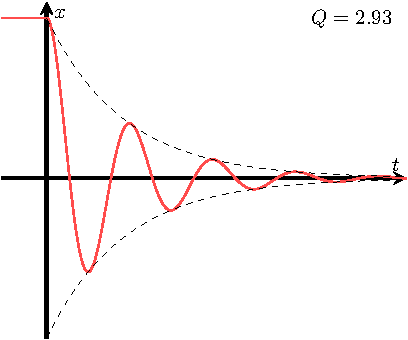
\includegraphics[width=.7\linewidth, draft=true]{carac-ra-3}
			      }{%
				      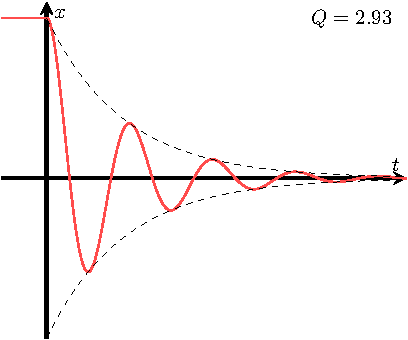
\includegraphics[width=.7\linewidth]{carac-ra-3}
			      }%
			      \captionof{figure}{%
				      Tracé solution $Q \approx 3$. \protect\pt{1}\psw{+}\protect\pt{1}
			      }%
		      \end{center}
		      \vspace*{-20pt}
	      \end{isd}
	      \vspace*{-30pt}
\end{enumerate}

\ifstudent{%
	\begin{tikzpicture}[remember picture, overlay]
		\node[anchor=north west, align=left]
		at ([shift={(1.4cm,0)}]current page.north west)
		{\\[5pt]\Large\bfseries Nom~:\\[10pt]\Large\bfseries Prénom~:};
		\node[anchor=north east, align=right]
		at ([shift={(-1.5cm,-17pt)}]current page.north east)
		{\Large\bfseries Note~:\hspace{1cm}/20};
	\end{tikzpicture}
}%

\end{document}
